\documentclass{note}
\usepackage{mathptm,mydef,myenv,alltt}
\usepackage[right]{lineno}
%\usepackage{MinionPro}
\usepackage{color}
%\usepackage[scaled]{beramono}
%\usepackage[scaled]{ulgothic}
%\usepackage[ocr-a]{ocr}
%\usepackage{ocr}
%\usepackage{courier}
\usepackage[all]{xy}
\renewcommand{\ttdefault}{txtt}
\usepackage[T1]{fontenc}
\usepackage{graphicx}
\DeclareGraphicsExtensions{.png}

\usepackage{hyperref}
\hypersetup{
    colorlinks,
    citecolor=black,
    filecolor=black, 
    linkcolor=blue,
    urlcolor=black
}

%\setlength\oddsidemargin{-1.5cm}
%\setlength\evensidemargin{-1.5cm}
%\setlength\textwidth{19.3cm}
%\addtolength\topmargin{-1cm}
%\addtolength\textheight{2cm}
%\addtolength\columnsep{0.2cm}
%\newtheorem{theorem}{Theorem}
%\theoremstyle{definition}
%\newtheorem{definition}[theorem]{Definition}
%\def\EE{\mbox{\eufm{}E}}1

\begin{document}
\small


%\title{\large\bf{}\textcolor{blue2}{Modem Design: UVM-to-UVMA Migration: Update \#2}}
\title{\large\bf{}\textcolor{blue2}{Modem Design: UVM-to-UVMA Migration:
    Update \#3}}
%\author{Cheoljoo Jeong}
%% $$\xy
%% %\vtop{\vbox{
%% \xygraph{!{0;/r0.7pc/:} !{\vover}[u]
%%   !{\hcap[-2]} [d] !{\vover-} [ruu] !{\hcap[2]}}
%% %}\smallskip}
%% \endxy$$
%% }
\date{}
%\date{\normalsize\today}
\maketitle

\tableofcontents

\linenumbers
\section{Overview}
%\subsection{Block diagram}
%\centerline{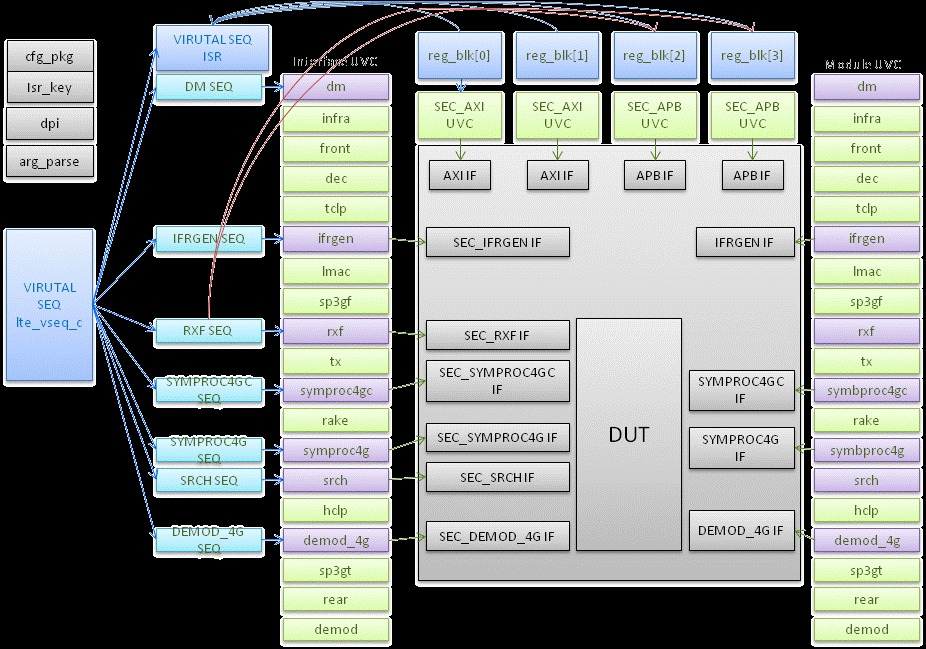
\includegraphics[width=12cm]{pics/modem}}

\subsection{Target files}
The following files are chosen by Yungi Um for migration. (files in \textcolor{red2}{RED} are available in VCAD chamber)
\bit
\w \bb{Common interface}:
   \bit
  \w \textcolor{red2}{\bb{sec\_modem/lib/common/common\_intf.sv}}
  \eit
\w \bb{Interfaces}:
  \bit
  \w \textcolor{red2}{\bb{sec\_modem/lib/rxf/rxf\_intf.sv}}
  \w \bb{sec\_modem/lib/symbproc4g/symbproc4g\_intf.sv}
  \w \textcolor{red2}{\bb{sec\_modem/lib/symbproc4gc/symbproc4gc\_intf.sv}}
  \w \textcolor{red2}{\bb{sec\_modem/lib/demod\_4g/demod\_4g\_intf.sv}}
  \w \bb{sec\_modem/lib/ifrgen/ifrgen\_intf.sv}
  \w \bb{sec\_modem/lib/dm/dm\_intf.sv}
  \w \bb{uvc/sec\_dm/v201408/sv/sec\_dm\_intf.sv}
  \w \bb{uvc/sec\_demod/v201408/sv/sec\_demod\_intf.sv}
  \w \bb{uvc/sec\_rxf/v201408/sv/sec\_rxf\_intf.sv}
  \eit
\w \bb{Interface instantiations}:
  \bit
  \w \bb{sec\_modem/tb/top/intf\_inst.sv}
  \eit
\w \bb{Drivers}:
  \bit
  \w \textcolor{red2}{\bb{uvc/sec\_rxf/v201408/sv/sec\_rxf\_driver.sv}}
  \eit
\w \bb{Monitors}:
  \bit
  \w \textcolor{red2}{\bb{sec\_modem/lib/common/base\_lib\_mon.sv}}
  \w \textcolor{red2}{\bb{sec\_modem/lib/symbproc4gc/symbproc4gc\_mon.sv}}
  \eit
\w \bb{Sequences}:
  \bit
  \w \bb{uvc/sec\_modem/lib/rxf/rxf\_\{seq,vseq\}\_lib.sv}
  \w \bb{uvc/sec\_modem/lib/symbproc4g/symbproc4g\_\{seq,vseq\}\_lib.sv}
  \w \bb{uvc/sec\_modem/lib/symbproc4gc/symbproc4gc\_\{seq,vseq\}\_lib.sv}
  \w
  \textcolor{red2}{\bb{uvc/sec\_modem/lib/demod\_4g/demod\_4g\_\{seq,vseq\}\_lib.sv}}
  (only seq\_lib given)
  \w \bb{uvc/sec\_modem/lib/dm/dm\_\{seq,vseq\}\_lib.sv}
  \w \bb{uvc/sec\_modem/lib/ifrgrn/ifrgen\_\{seq,vseq\}\_lib.sv}
  \eit
\w \bb{Checkers}:
  \bit
  \w \textcolor{red2}{\bb{checkers/demod\_4g/NonCol\_Compare.inc}}
  \w \textcolor{red2}{\bb{checkers/demod\_4g/compare\_fdi.inc}}
\w \textcolor{red2}{\bb{checkers/demod\_4g/Pbch\_Compare.inc}}
\w \textcolor{red2}{\bb{checkers/demod\_4g/compare\_iw\_rcal\_done.inc}}
\w \textcolor{red2}{\bb{checkers/demod\_4g/ce\_pp\_compare.inc}}
\w \textcolor{red2}{\bb{checkers/demod\_4g/compare\_mmsewg.inc}}
\w \textcolor{red2}{\bb{checkers/demod\_4g/ce\_y\_compare.inc}}
\w \textcolor{red2}{\bb{checkers/demod\_4g/compare\_tdi.inc}}
\w \textcolor{red2}{\bb{checkers/demod\_4g/compare\_ToneDemapper.inc}}
\w \textcolor{red2}{\bb{checkers/demod\_4g/drs\_dmrs\_ext.inc}}
\w \textcolor{red2}{\bb{checkers/demod\_4g/compare\_chbridge\_mimoout.inc}}
\w \textcolor{red2}{\bb{checkers/demod\_4g/fdagc\_checker.inc}}
\w \textcolor{red2}{\bb{checkers/demod\_4g/compare\_chbridge\_mimooutCCD.inc}}
\w \textcolor{red2}{\bb{checkers/demod\_4g/fft\_checker.inc}}
\w \textcolor{red2}{\bb{checkers/demod\_4g/compare\_chbridge\_mimooutCCDHICH.inc}}
\w \textcolor{red2}{\bb{checkers/demod\_4g/front\_out\_checker.inc}}
\w \textcolor{red2}{\bb{checkers/demod\_4g/compare\_chbridge\_mimooutPBCH.inc}}
\w \textcolor{red2}{\bb{checkers/demod\_4g/pdp\_checker.inc}}
\w \textcolor{red2}{\bb{checkers/demod\_4g/compare\_chbridge\_pdcch\_llr.inc}}
\w \textcolor{red2}{\bb{checkers/demod\_4g/sinr\_checker.inc}}
\w \textcolor{red2}{\bb{checkers/demod\_4g/compare\_csi\_postproc.inc}}
\w \textcolor{red2}{\bb{checkers/demod\_4g/tc\_checker.inc}}
\w \textcolor{red2}{\bb{checkers/demod\_4g/compare\_csi\_preproc.inc}}
\eit
\eit


\subsection{Code organization}
The following ``initial'' code organization is assumed.
\subsubsection{TB}
\begin{alltt}
  module incr_top;
    //`include "env_intf_inst.sv"
    intf intf(.nReset(top.nReset), .SystemClock(top.SystemClock, .*);

    // interface instantiations
    // interface could be instantiated either in DUT or TB initially;
    // if instantiated inside DUT, should be set as dutexcl to map it to SW
    // initially; eventually, H-interface portion of rxf_intf will be mapped 
    // to HW 
    rxf_intf rxf_intf(.nReset(top.nReset),
                      .SystemClock(top.SystemClock),
                      .clk(top.clkrst_if.clk245),
                      .clkx2(top.clkrst_if.clk245),
                      .clkx4(top.clkrst_if.clk245),
                      .reset_n(top.clkrst_if.rsn));
    
    initial begin
      uvm_config_db#(virtual intf)::set(null, "uvm_test_top.*", "vintf", 
                                        incr_top.intf);
    end
  endmodule

\end{alltt}

\subsubsection{DUT}
\begin{alltt}
  module top;
    // clock/reset interface
    clkrst_intf clkrst_if(...);

    // DUT wrapper
    dut dut;
  endmodule
  module dut;
    Modem A_Modem;
  endmodule
  module A_Modem
  endmodule
\end{alltt}

% SECTION: Remodeling for Simulation Acceleration
%\section{Remodeling for Simulation Acceleration}
Code in UVC/TB uses constructs which are generally considered non-RTL.
For UVMA migration, some of the code in TB must be moved into interfaces,
which in turn, are mapped to HW. 
So, those constructs need to be remodeled so that they can be synthesized by
UXE. 

\vspace*{0.2cm}

\noindent\textcolor{red2}{NOTE: Please do not remodel for now.}

\subsection{Level-sensitive sequence controls}
The following statement
\begin{verbatim}
FROM:
  event ev;
  wait(ev.triggered);

TO:
  @(ev);
\end{verbatim}

\subsection{Clock-gating expressions}
\bit
\w \bb{CASE \#1}:
\begin{verbatim}
FROM:
  always @(posedge clk iff cond) begin
    S1
  end

TO:
  always @(posedge clk) begin
    if (cond) begin
      S1
    end
  end
\end{verbatim}

\w \bb{CASE \#2}:
\begin{verbatim}
FROM:
  initial 
    forerver
      @(posedge clk iff cond);
      S1
    end

TO:
  always @(posedge clk) begin
    if (cond) begin
      S1
    end
  end
\end{verbatim}
\eit

\paragraph{Forever statement inside tasks}
One design pattern used in many parts is the following:
\begin{verbatim}
  initial 
    fork
      foo(0);
      foo(1);
    join
 
  task foo(int v);
    forever begin
      @(posedge clk iff cond);
      if (expected[i] != values[v][i])
        $display("error");
    end
  endtask

\end{verbatim}
Above code is effectively the same as the following, where ``\verb+forerver+''
can be changed to ``\verb+always+''. (The latter is macro-based syntactic transformation while the former is more programmatic.)
\begin{verbatim}
  generate for (i = 0; i < 1; i++) 
    always @(posedge clk iff cond);
      if (expected[i] != values[v][i])
        $display("error");
    end
  endgenerate
\end{verbatim}




\section{Migration Steps}

\subsection{STEP \#1: From signal-based to transaction-based}
\subsubsection{Action items}
\bit
\w Move all tasks used inside DRIVER and MONITOR into interfaces. 
   In particular, 
   \bit
   \w \verb+drive_transfer+ task should be moved out of DRIVER class
       and put inside target SV interface
      \bit
      \w See SECTION~5:STEP\#1, for details.
      \eit
   \w \verb+collect_type0+ and \verb+collect_type1+ task should be
      moved out of MONITOR class and put inside target SV interface
      \bit
      \w See SECTION~6:STEP\#1, for details.
      \eit
   \eit
\eit
\subsubsection{Notes}
\bit
\w At this point, no need to worry about synthesizability,
 since the SV interface will be still in SW-space. If the interface, say
 \verb+sec_rxf_intf+ is instantiated under DUT (or we can still leave
 them under INCR\_TOP), then we should map it to
 SW by providing IXCOM option \verb|+dutexcl+sec_rxf_intf|. 
\eit

\subsection{STEP \#2: Clean-up common interface}
\subsubsection{Action items}
\bit
\w \bb{COMMON\_INTF}: Split \verb+common_intf.sv+ into two parts:
  \verb+common_intf_S.sv+ and \verb+common_intf_H.sv+. 
   \bit
   \w \verb+common_intf_S.sv+ will contain all objects which is
     non-synthesizable or is non-essential for DUT computation or checking
   \w \verb+common_intf_H.sv+ will contain all objects which are actually
     driven DUT and will be used inside DUT (especially for checking, etc.)
   \w all SV interfaces which include \verb+common_intf.sv+ must be changed 
   so that they will include both \verb+common_intf_H.sv+ and
   \verb+common_intf_S.sv+. 
      \bit
      \w See SECTION~3, for details.
      \eit
   \eit
\w \bb{CHECKERS}: Move checkers into DUT
\eit
\subsubsection{Notes}
\bit
\w Entire checker module should be included into DUT.
  Moving checkers into DUT is a good exercise for STEP \#3 and \#4. Also,
  would give good introduction how to make non-synthesizable module into 
  PXP HW.
\w \textcolor{red2}{After STEP \#2, HW-run MUST pass}.
\eit

\subsection{STEP \#3: Split S-interface and H-interface}
\subsubsection{Action items}
\bit
\w \bb{STEP \#3.1: Split interfaces}: Now, each actual interface should be split into S-interface
and H-inteface. For example, \verb+rxf_intf.sv+ should be split into
\verb+rxf_intf_S.sv+ and \verb+rxf_intf_H.sv+. 
   \bit
   \w First, for each sig1nal defined in SV interface, decide where to put it: 
    HW (\verb+rxf_intf_H+) or SW (\verb+rxf_intf_S+)
   \w Next, for each process (INITIAL or ALWAYS) and task/function, decide
   where to put it:
    HW (\verb+rxf_intf_H+) or SW (\verb+rxf_intf_S+)
      \bit
      \w Some process touches both signals in HW (\verb+rxf_intf_H+) and
      signals in (\verb+rxf_intf_S+). 
      \w  Then, such process need to be rewritten so that it will be split
      into two parts: HW-part, and SW-part. 
      \w Also, some logic may need to be inserted to connect the HW-part of the
      process and SW-part of the process.
      \eit
   \w \verb+rxf_intf_H.sv+ will be compiled by IXCOM (in DUT compilation)
     \bit
     \w But still, we will map \verb+rxf_intf_H+ into SW since it will still
        contain nonsynthesizable constructs
     \w \verb+rxf_intf_H+ interface should only include \verb+common_intf_H.sv+
     \eit
   \w \verb+rxf_intf_S.sv+ will be compiled by IES (in TB compilation)
     \bit
     \w \verb+rxf_intf_S+ interface should only include
     \verb+common_intf_S.sv+
     \eit
   \eit
\w \bb{STEP \#3.2: Remove non-synthesizable constructs from H-interfaces}:
  \bit
  \w All uses of non-synthesizable objects in H-interface (e.g. queues,
  dynamic arrays, etc.) should be remodeled using synthesizable objects.
  \w After this SUBSTEP, remove all \verb|+dutexcl+<intf>| options. 
    Make sure IXCOM compilation works and all
    H-interfaces are mapped to HW. HW-run or SW-run would not pass since we
    haven't connected S-interface and H-inteface yet. 
  \eit
\w \bb{STEP \#3.3: Connect S-interface with H-interface using DPIMAP}:
  \bit
  \w After H-interfaces are mapped to HW, even SW-run would not pass. To make
  this pass, we need to bridge two using DPIMAP.
  \w Also, any memory transfer should be modified to use
  \verb+dpiMap::put/getBytes()+ function calls.
  \eit
\eit
\subsubsection{Notes}
\bit
\w \textcolor{red2}{After STEP \#3.1, HW-run MUST pass}.
\w \textcolor{red2}{After STEP \#3.2, SW-run MUST pass}.
\w \textcolor{red2}{After STEP \#3.3, HW-run MUST pass}.
\eit
\subsection{STEP \#4: Performance Optimization}
\subsubsection{Action items}
\bit
\w Iteration: profiling and performance optimization.
\eit


\section{Common Interface: common\_intf.sv}
%% Every interface includes \verb+common_intf.sv+
%% (i.e. \verb+`include common_intf.sv+).
%% Common interfaces contain objects for
%%   \bit
%%   \w reference (golden) data 
%%   \w signals to mirror DUT signals
%%   \w signals to control error checking (e.g. enable/disable check, etc.)
%%   \eit
%% Later, actual interfaces (which include this common interface) add more
%% signals, and initial/always processes to perform the following:
%%   \bit
%%   \w read reference data from files
%%   \w continous assignments to mirror DUT signals into interface signals
%%   \w control signals for error checking
%%   \eit
%% Signals defined in common interfaces are used in MONITORs and DRIVERS
Common interface objects defined in
\verb+common_intf.sv+ can be classified into two: a) objects to put into HW
and b) objects to put into SW. 

For example, \verb+check_data+ which are bound to
actual DUT signals should be put into HW for performance. If we put it in SW, every time the corresponding DUT signal changes, the value change should be propagated to \verb+check_data+ which is sitting in SW.
However, some objects should be put into SW either because they cannot be 
synthesized in HW (e.g. strings) or they actually are not needed for 
DUT computation -- \verb+check_int_key_name+ appears to fall into this category.  
\vspace*{0.3cm}

{\bf{}\noindent{NOTE:} From now on, when a code is displayed, the following color coding is used.}
\bit
\w \textcolor{red2}{\bf{}RED means that the code should be put into HW for performance}
\w \textcolor{blue2}{\bf{}BLUE means that the code should be put in SW, either because it's non-synthesizable or there's little benefit in putting it to HW.}
\w \textcolor{green2}{\bf{}GREEN means that it's not clear where to put the code.}
\w \bb{BOLD comments were added by Cheoljoo} and comments in normal font is original comment in the code.
\eit

\subsection{CODE}
\begin{alltt}
    \textcolor{green2}{\textbf{// (i) PULSE GEN}
    \textbf{//   - Q: what is the purpose of this pulse signal? also, where are the loads of this signal?}
    \textbf{//        why vclk?}
    bit vclk;
    always #2 vclk = ~vclk;
    `define INT_PULSE_GEN(NAME,SRC) \textbackslash
      bit r``NAME; \textbackslash
      always @ (posedge vclk) r``NAME <= SRC; \textbackslash
      wire NAME``Pulse = SRC&~r``NAME;}

    \textcolor{blue2}{\textbf{// (ii) METAINFO of REFERNCE (GOLDEN) DATA: filled up from FILE at time 0 and compared against 
    //      DUT-generated data later
    //   - it appears that folowing BLUE code are mostly for logging purpose and  put only into q
    //     SW-side (e.g. S-interface) and access them only from SW-side
    //   - there are MAX_CHECK_NUM check points, where each check point is specified by a single file
    //   - MAX_CHECK_NUM is an interface parameter
}    string check_point_name[MAX_CHECK_NUM];

    // the reference file name
    string check_ref_file_name[MAX_CHECK_NUM];

    // reference file type (0: 1 column, non zero: 2 columns)
    // 1: (i,q) pair
    // 2: (addr,data) pair
    int check_ref_file_type[MAX_CHECK_NUM];

    // reference file existence
    int check_ref_file_exists[MAX_CHECK_NUM];

    // reference data size (only for collect_type1)
    int check_ref_data_max_num[MAX_CHECK_NUM];
    initial foreach (check_ref_data_max_num[i]) check_ref_data_max_num[i] = -1;

    // key information to extract reference data from file
    string check_int_key_name[MAX_CHECK_NUM][$];
    int check_int_key_value[MAX_CHECK_NUM][$];
    string check_str_key_name[MAX_CHECK_NUM][$];
    string check_str_key_value[MAX_CHECK_NUM][$];}

    
    \textcolor{red2}{\textbf{// (iii) CHECK_CLOCK: used to clock checking processes, etc.}
    \textbf{//   - driven from DUT (Q: can you confirm?)}
    \textbf{//   - used in TB; uses of CHECK_CLOCK are:}
    \textbf{//     . MONITOR code uses this clock to fetch one DUT output item, which is put into a queue }
    \textbf{//       inside a transaction}
    \textbf{//     . for updating CHECK_REF_DATA_IDX inside a process in interfaces, (CHECK_REF_DATA_IDX}
    \textbf{//       value is eventually used inside MONITOR code, to number DUT output item}
    // clock used for capturing the sample
    logic check_clk[MAX_CHECK_NUM];
  
    \textbf{// Q: when CHECK_CLK_SKIP_NUM is NOT 0, where do we get the non-0 value?}
    \textbf{//   - is it a constant or value is read from a file?}
    // number of clocks we should skip after capturing the sample (usually 0)
    int check_clk_skip_num[MAX_CHECK_NUM];

    \textbf{// (iv) CHECK_START: indicates that now DUT emits outputs that need to be checked}
    \textbf{//   - driven from DUT}
    \textbf{//   - on CHECK_START, TB code will populate parameters of the given check point.}
    \textbf{//     . after parameters are set, CHECK_PARAM_SET_END will be set}
    \textbf{//   - MONITOR code (collect_type) waits for CHECK_START and CHECK_PARAM_SET_END, and then}
    \textbf{//     start to fetch DUT output item one by one into transaction}
    // signal indicating the start of the related logic (once or multiple times throughout simulation)
    // if we use multiply-generated start signal, should use "collect_type0" function at monitor.
    // else if we use one-time-generated start singal, should use "collect_type1" function at monitor.
    logic check_start[MAX_CHECK_NUM];

    \textbf{// (v) CHECK_DATA_EN: level signal which is asserted while DUT generates output items}
    \textbf{//   - processes clocked on CHECK_CLK are guarded by this}
    // in-time data enable signal used for capturing the sample
    logic check_data_en[MAX_CHECK_NUM];

    \textbf{// (vi) CHECK_DATA: actual DUT output items}
    \textbf{//   - driven through XMR}
    // DUT signal to be captured
    logic [127:0] check_data[MAX_CHECK_NUM];
    logic [127:0] check_data_i[MAX_CHECK_NUM];
    logic [127:0] check_data_q[MAX_CHECK_NUM];}

    \textcolor{blue2}{\textbf{// (vii) CHECK_MASK}
    \textbf{//  - mostly constant value (driven through cont asgn}
    \textbf{//  - only read by TB (in collect_type in MONITOR)}
    \textbf{//  - Q: can you confirm that it's only used in collect_type task?}
    // this is used for masking the invalid bit within 128-bit.
    logic [127:0] check_mask[MAX_CHECK_NUM];}

    \textcolor{red2}{\textbf{// (viii) CHECK_REF_DATA_IDX: during checking, multiple output items to be checked are }
    \textbf{// generated by DUT, this index is used to number them}
    \textbf{//   - typically initialized to 0 on CHECK_START}
    \textbf{//   - incremented by 1 on CHECK_CLOCK edge iff CHECK_DATA_EN}
    \textbf{//   - only used in collect_type task in MONITOR code}
    \textbf{//   - still, better to update this value in HW since the update logic is clocked; }
    \textbf{//     if we update this value in SW, we need to stop on every CHECK_CLK posedge}
    // symbol index within key group in testvector synchronizing with the currently being 
    // captured DUT data
    int check_ref_data_idx[MAX_CHECK_NUM];}

    \textcolor{red2}{\textbf{// (ix) CHECK_DONE: opposite of CHECK_START
    //   - used to indicate the end of one CHECK BURST
    //   - see collect_type0 code in MONITOR how it's used
    //   - for performance, we better put this to HW; for details, see section on MONITOR}
    // if some burst processing has its start-done pair, we should describe its done signal.
    // this is only valid when multiple start signals exist ("collect_type0")
    logic check_done[MAX_CHECK_NUM];

    // if some burst processing generates multiple done signals at a single start signal, 
    // we should define the number of done signal.
    // this is only valid when multiple start signals exist  ("collect_type0")
    int check_done_num[MAX_CHECK_NUM];}

    \textcolor{blue2}{\textbf{// (x) CHECK_PARAM_SET_END
    //   - on CHECK_START, some SW-code for inserting ``markers'', which marks the beginning of new
    //     check data is inserted
    //   - CHECK_PARAM_SET_END is triggered to tell such insertion is finished
    //   - after CHECK_PARAM_SET_END (and CHECK_START) actually, collecting begins}
    // we should trigger this event, when we finish setting all parameters of checking point.
    // this starts monitor to capture the samples.
    event check_param_set_end[MAX_CHECK_NUM];}

    \textcolor{red2}{\textbf{// (xi) CHECKER_ON: looks like another guard which enables/disables CHECKING}
    bit checker_on;
    // this indicates whether this block is enabled.
    // we trigger on at body task of monitor.}

    \textcolor{green2}{\textbf{// (xi) TEST_ON}
    \textbf{//   - Q: what is this for?}
    \textbf{//   - Q: why is the value set after #5000?}
    \textbf{//   - if we need to put this to HW, may be need to remodel as in:
    //     S_intf: initial #5000ns H_intf.set_test_on();
    //     H_intf: function void set_test_on; test_on = checker_on; endfuncion}
    bit test_on;
    // this indicates whether reset is released.
    initial #5000ns test_on = checker_on;}
\end{alltt}

\subsection{Details}
\bit
\w \bb{STEP \#1}: Split \verb+common_intf.sv+ into two: one for SW-side, the other for HW-side
  \ben
  \w Create two files: \verb+common_intf_S.sv+ and \verb+common_intf_H.sv+.
\begin{alltt}
  // common_intf_S.sv
\end{alltt}
  \w Change the original \verb+common_intf.sv+ file.
\begin{verbatim}
  `include "common_intf_S.sv"
  `include "common_intf_H.sv"
\end{verbatim}
  \een
\w \bb{STEP \#2}: No further steps needed for this file. Later, when we split an actual interface into S-interface and H-interface, we can have S-interface include \verb+common_intf_S.sv+ and have H-interface include \verb+common_intf_H.sv+.
\eit


\section{INTERFACES}
Interfaces contain objects and processes.  For acceleration, we need to split the set of objects and processes into two: one for HW and the other for SW.
For this, remodeling may be needed. Also, code which bridges between HW and 
SW objects/processes may need to be added. 

\subsection{demod\_4g\_intf.sv}
%\input{code/demod_4g_intf.sv}
\bit
\w This interface is mostly empty.
\eit

\subsection{symbproc4gc\_intf.sv}
%\input{code/symbproc4gc_intf.sv}
\bit
\w \bb{SETUP}: 
   \bit
   \w There are 49 check items: \verb+Check [0]+ through \verb+Check [48]+.
   \w For each check item there are code which performs following (consider
   \verb+Check [0]+ for example):
 \begin{alltt}
  \textcolor{red2}{\textbf{// binds real ``DUT signals'' to ``generic'' interface signals; should be put into HW
     - Q: Can you confirm sp4gc_Clk245, sp4gc_BchStrt are DUT signals? How are they driven? 
          In a continuous assignment such as "assign sp4gc_Clk245 = dut.x.clk"?}
  assign  check_clk[0]            = sp4gc_Clk245;
  initial check_ref_file_name[0]  = $sformatf("lspcch_dscr_a0301_in.txt");
  assign  check_start[0]          = sp4gc_BchStrt;
  assign  check_clk_skip_num[0]   = 0;
  assign  check_data_en[0]        = sp4gc_BchDataEn;
  assign  check_mask[0]           = 6'h3f;
  assign  check_done_num[0]       = 1;
  assign  check_done[0]           = sp4gc_WagWrDone;
  assign  check_data[0]           = sp4gc_BchData;}

  \textcolor{blue2}{\textbf{// most of the following code should be executed in SW space; either
  //   i) can be transformed into}
  \textbf{//        always @(posedge check_start[0] iff checker_on)}
  \textbf{//          do_check_param_set(HenbTtiOn, ...);}
  \textbf{//      where do_check_param_set is defined in SW (say, common_intf_sw.sv)
  // or 
  //   ii) just put the entire process into S-interface and set check_start, checker_on, 
  //       sp4gc_* signals as export_read. If value changes are frequent on these signals, 
  //       i) would be more efficient. }
  always@(posedge check_start[0] iff checker_on)
  begin
    if(sp4gc_PbchDecOn&&sp4gc_start_cnt==0)
      check_ref_data_idx[0] = 0;
    check_int_key_name[0].delete();
    check_int_key_value[0].delete();
    check_str_key_name[0].delete();
    check_str_key_value[0].delete();

    if (sp4gc_EicicOn) begin
      check_point_name[0]     = $sformatf("lspcch_a0301_in_bch (for Regen)");
    end else if (HenbTtiOn) begin
      check_point_name[0]     = $sformatf("lspcch_a0301_in_bch (for Henb)");
    end else begin
      check_point_name[0]     = $sformatf("lspcch_a0301_in_bch");
    end

    if (sp4gc_EicicOn) begin
    end else begin
      if (HenbTtiOn) begin
        check_int_key_name[0].push_back("asfr");
        check_int_key_value[0].push_back(10);
      end else begin
        check_int_key_name[0].push_back("fr");
        check_int_key_value[0].push_back(fr_idx_pbch);
      end
    end

    check_int_key_name[0].push_back("cc");
    check_int_key_value[0].push_back(0);

    if(sp4gc_PbchDecOn) begin
      check_str_key_name[0].push_back("chan");
      check_str_key_value[0].push_back("PBCH");
      if (sp4gc_oPdcchSibUnknown) begin
        check_int_key_name[0].push_back("decGrp");
        check_int_key_value[0].push_back(sp4gc_oPdcchSibUnknownIdx-1);
      end else begin
        check_int_key_name[0].push_back("decGrp");
        check_int_key_value[0].push_back(sp4gc_pbch_decgrp);
      end
    end
      ->check_param_set_end[0];
  end}

  \textcolor{red2}{\textbf{// should be put into HW}
  always@(posedge sp4gc_Clk245 iff checker_on)
    if(sp4gc_CchDecDone)
      sp4gc_start_cnt <= 0;
    else if(check_done[0])
      sp4gc_start_cnt <= sp4gc_start_cnt+1;

  always@(posedge sp4gc_Clk245 iff checker_on)
    if(check_data_en[0])
      check_ref_data_idx[0] <= check_ref_data_idx[0]+1;}
 \end{alltt}
   \eit
\w \bb{STEP \#1}: Create a task to be used between S-interface and H-interface. 
  \bit
  \w For each \verb+Check[+$i$\verb+]+, change the BLUE code as follows.
 \begin{alltt}
  \textbf{// add appropriate types for task parameters}
  \textbf{//   - will be put into S-interface, in a later STEP}
  function void do_check_param_set(input sp4gc_EicicOn, HenbTtiOn, sp4gc_PbchDecOn,
                                   sp4gc_oPdcchSibUnknown);
    check_int_key_name[0].delete();
    check_int_key_value[0].delete();
    check_str_key_name[0].delete();
    check_str_key_value[0].delete();
    if (sp4gc_EicicOn) begin
      check_point_name[0]     = $sformatf("lspcch_a0301_in_bch (for Regen)");
    end else if (HenbTtiOn) begin
      check_point_name[0]     = $sformatf("lspcch_a0301_in_bch (for Henb)");
    end else begin
      check_point_name[0]     = $sformatf("lspcch_a0301_in_bch");
    end

    if (sp4gc_EicicOn) begin
    end else begin
      if (HenbTtiOn) begin
        check_int_key_name[0].push_back("asfr");
        check_int_key_value[0].push_back(10);
      end else begin
        check_int_key_name[0].push_back("fr");
        check_int_key_value[0].push_back(fr_idx_pbch);
      end
    end

    check_int_key_name[0].push_back("cc");
    check_int_key_value[0].push_back(0);

    if(sp4gc_PbchDecOn) begin
      check_str_key_name[0].push_back("chan");
      check_str_key_value[0].push_back("PBCH");
      if (sp4gc_oPdcchSibUnknown) begin
        check_int_key_name[0].push_back("decGrp");
        check_int_key_value[0].push_back(sp4gc_oPdcchSibUnknownIdx-1);
      end else begin
        check_int_key_name[0].push_back("decGrp");
        check_int_key_value[0].push_back(sp4gc_pbch_decgrp);
      end
    end
      ->check_param_set_end[0];
  endfunction

  \textbf{// Always process will be put into HW}
  \textbf{//   - will be put into H-interface, later}
  always@(posedge check_start[0]) begin
    if (checker_on) begin
      if(sp4gc_PbchDecOn&&sp4gc_start_cnt==0)
        check_ref_data_idx[0] = 0;
      \textbf{do_check_param_set(sp4gc_EicicOn, HenbTtiOn, sp4gc_PbchDecOn, sp4gc_oPdcchSibUnknown);}
    end
  end
 \end{alltt}
 \w Validate the code change.
 \eit
\w \bb{STEP \#2}: Partition the code into H-interface code and S-inteface code.
  \bit
  \w To be continued.
  \eit
\eit

\subsection{rxf\_intf.sv}
%\input{code/rxf_intf.sv}
%% \bit
%% \w \bb{start condition}
%%   \bit
%%   \w from DRV: RX\_START
%%   \w from DUT: \_3gf\_RXStart, \_3gt\_RXStart
%%   \eit
%% \eit


%%\bit
%% \w \bb{CODE}: Consider the following code fragment.
%%  \begin{alltt}
%%    logic   [119:0]       DUT_IntCpu;

%%    // modem primary IO interrupts
%%    `INT_PULSE_GEN (IntFreqShift,DUT_IntCpu[65])

%%    // ---------------------------------------
%%    // signals for driving L1
%%    // ---------------------------------------
%%    // Common
%%    logic [MAX_CH_NUM-1:0]  Tclk;
%%    logic                  GapRfStartTick, GapRfEndTick;
%%    logic   [3:0]          GapInfo[3];
%%    logic   [15:0]         ClkCount[3];

%%    logic                   PnClk2En_3GF;
%%    // Start signal from DUT
%%    logic                   _3gf_RxStart;
%%    logic                   _3gt_RxStart;
%%    // Start signal from DRV
%%    logic                   RX_START;
%%    // Monitoring signal
%%    bit [3:0] checker_3gf_start;
%%    bit checker_3gt_start;

%%    // 4G DVGA update
%%    bit                  RTG_CLK;
%%    logic   [3:0]        TTI_INDEX[3];
%%    logic   [2:0]        RxfTtiTick;
%%    logic   [2:0]        wTTI_TICK;
%%    logic   [2:0]        rTTI_TICK;
%%    logic   [2:0]        rTTI_INDEX_ON;

%%    always @(posedge RTG_CLK or negedge reset_n) begin
%%       if (!reset_n) begin
%%          rTTI_TICK <= 0;
%%          rTTI_INDEX_ON <= 0;
%%       end
%%       else begin
%%          rTTI_TICK <= wTTI_TICK;
%%          for (int i = 0; i < 3; i++)
%%             if (RxfTtiTick[i])
%%                rTTI_INDEX_ON[i] <= 1;
%%       end
%%    end


%%    // `INT_PULSE_GEN (IntBtfdEnd,DUT_IntCpu[34])
%%    // ---------------------------------------
%%    // + argument parsing
%%    // ---------------------------------------
%%    int front_rxf_uvc_cfg;
%%    int demod_rake_uvc_cfg;
%%    int demod_tclp_uvc_cfg;
%%    int check_3gf_rxf_start_offset[4] = '{12,12,12,12};
%%    int check_3gf_adcnum4fa[4];
%%    string rat_mode_cfg;
%%    string vec_dir;

%%    initial begin
%%       // check forcing argument
%%       if ($value$plusargs("front_rxf_uvc_cfg=%d", front_rxf_uvc_cfg));
%%       if ($value$plusargs("demod_rake_uvc_cfg=%d", demod_rake_uvc_cfg));
%%       if ($value$plusargs("demod_tclp_uvc_cfg=%d", demod_tclp_uvc_cfg));
%%       if ($value$plusargs("check_3gf_rxf_start_offset0=%d",
%%                                 %check_3gf_rxf_start_offset[0]));
%%       if ($value$plusargs("check_3gf_rxf_start_offset1=%d",
%%                                 %check_3gf_rxf_start_offset[1]));
%%       if ($value$plusargs("check_3gf_rxf_start_offset2=%d",
%%                                 %check_3gf_rxf_start_offset[2]));
%%       if ($value$plusargs("check_3gf_rxf_start_offset3=%d",
%%                                 %check_3gf_rxf_start_offset[3]));
%%       if ($value$plusargs("check_3gf_adcnum4fa0=%d", %check_3gf_adcnum4fa[0]));
%%       if ($value$plusargs("check_3gf_adcnum4fa1=%d", %check_3gf_adcnum4fa[1]));
%%       if ($value$plusargs("check_3gf_adcnum4fa2=%d", %check_3gf_adcnum4fa[2]));
%%       if ($value$plusargs("check_3gf_adcnum4fa3=%d", %check_3gf_adcnum4fa[3]));
%%       if ($value$plusargs("rat_mode_cfg=%s", rat_mode_cfg));
%%       if ($value$plusargs("vec_dir=%s", vec_dir));

%%       for (int i=0; i<4; i=i+1)
%%          $display("rf_check_offset[%d] = %d", i, %check_3gf_rxf_start_offset[i]);

%%       if (front_rxf_uvc_cfg == 'd1 ||
%%           front_rxf_uvc_cfg == 'd3 ||
%%           front_rxf_uvc_cfg == 'd4)
%%           checker_on = 1;
%%    end
%%    initial begin
%%       #1;
%%       if (rat_mode_cfg=="3gf") begin
%%         @ (posedge (demod_rake_uvc_cfg == 0 ? RX_START : _3gf_RxStart));
%%         fork
%%           begin @ (posedge Tclk[check_3gf_adcnum4fa[0]]); checker_3gf_start[0] = 1; end
%%           begin @ (posedge Tclk[check_3gf_adcnum4fa[1]]); checker_3gf_start[1] = 1; end
%%           begin @ (posedge Tclk[check_3gf_adcnum4fa[2]]); checker_3gf_start[2] = 1; end
%%           begin @ (posedge Tclk[check_3gf_adcnum4fa[3]]); checker_3gf_start[3] = 1; end
%%         join
%%       end
%%       if (rat_mode_cfg=="3gt") begin
%%         @ (posedge (demod_tclp_uvc_cfg == 0 ? RX_START : _3gt_RxStart));
%%         @ (posedge Tclk[0]);
%%         checker_3gt_start = 1;
%%       end
%%    end

%%    // ------------------
%%    // checkers
%%    // ------------------
%%    // [0]: c0 a0
%%    // [1]: c0 a1
%%    // [2]: c1 a0
%%    // [3]: c1 a1
%%    // [4]: c2 a0
%%    // [5]: c2 a1
%%    // [6]: c3 a0
%%    // [7]: c3 a1
%%    logic [7:0] oFa0Rx0I;
%%    logic [7:0] oFa0Rx0Q;
%%    logic [7:0] oFa0Rx1I;
%%    logic [7:0] oFa0Rx1Q;
%%    logic [7:0] oFa1Rx0I;
%%    logic [7:0] oFa1Rx0Q;
%%    logic [7:0] oFa1Rx1I;
%%    logic [7:0] oFa1Rx1Q;
%%    logic [7:0] oFa2Rx0I;
%%    logic [7:0] oFa2Rx0Q;
%%    logic [7:0] oFa2Rx1I;
%%    logic [7:0] oFa2Rx1Q;
%%    logic [7:0] oFa3Rx0I;
%%    logic [7:0] oFa3Rx0Q;
%%    logic [7:0] oFa3Rx1I;
%%    logic [7:0] oFa3Rx1Q;
%%    `ifndef TEST_4G
%%    `ifdef _3G_OFFSET_FIND
%%       int check_3gf_rxf_free_cnt[4];
%%       bit [3:0] check_3gf_rxf_en;
%%       for (genvar i=0; i<4; i++)
%%          always @ (posedge PnClk2En_3GF iff checker_3gf_start[i]) begin
%%             check_3gf_rxf_free_cnt[i]++;
%%             if (check_3gf_rxf_free_cnt[i]>=check_3gf_rxf_start_offset[i])
%%                check_3gf_rxf_en[i] = 1;
%%          end

%%       int rxf_out_sample_num_3gf[3:0]; // for waveform check
%%       always @(negedge PnClk2En_3GF)
%%          for (int i=0; i<4; i++)
%%             rxf_out_sample_num_3gf[i] =
%%             check_3gf_rxf_free_cnt[i]-check_3gf_rxf_start_offset[i]+1;

%%       int check_3gf_Fptr[8],check_3gf_line_valid[8];
%%       string check_3gf_line[8],check_3gf_vec_dir[8],check_3gf_str0[8],
%%              check_3gf_str1[8];
%%       for (genvar i=0;i<8;i++) begin
%%          initial check_point_name[i] =
%%             $sformatf("rx_filter output @ (carrier:%0d, %antenna:%0d)",i/2,i%2);
%%          assign check_clk[i] = PnClk2En_3GF;
%%          initial begin
%%             #1;
%%             check_ref_file_name[i] =
%%             $sformatf("rxflt_dcr2_a0007_out3gf_a%0dc%0d.txt",i%2,i/2);
%%             void'($value$plusargs("vec_dir=%s", check_3gf_vec_dir[i]));
%%             check_ref_file_exists[i] = FILE_CHECK_LOCAL
%%             ($sformatf("%0s/%0s",check_3gf_vec_dir[i],check_ref_file_name[i]));
%%             if (check_ref_file_exists[i]) begin
%%                check_3gf_Fptr[i] = $fopen($sformatf("%0s/%0s",check_3gf_vec_dir[i],
%%                                           check_ref_file_name[i]),"r");
%%                check_ref_data_max_num[i] = 0;
%%                while ($fgets (check_3gf_line[i],check_3gf_Fptr[i])) begin
%%                   check_3gf_line_valid[i] = $sscanf (check_3gf_line[i],"%s %s",
%%                        check_3gf_str0[i],check_3gf_str1[i]);
%%                   if (check_3gf_line_valid[i] == 2)
%%                      check_ref_data_max_num[i]++;
%%                end
%%                $fclose (check_3gf_Fptr[i]);
%%             end
%%             check_int_key_name[i].push_back("fr");
%%             check_int_key_value[i].push_back(0);
%%             check_ref_file_type[i] = 1;
%%          end
%%          assign check_start[i] = (demod_rake_uvc_cfg == 0 ? RX_START : _3gf_RxStart) & 
%%                                  check_ref_file_exists[i];
%%          assign check_clk_skip_num[i] = 0;
%%          assign check_mask[i] = 8'hff;
%%          assign check_data_en[i] = check_3gf_rxf_en[i/2] & check_ref_file_exists[i];
%%          always @ (posedge check_start[i] iff checker_on) begin
%%             check_ref_data_idx[i] = 0;
%%             ->check_param_set_end[i];
%%          end
%%          always @ (posedge check_clk[i] iff check_data_en[i] & checker_on)
%%             #1 check_ref_data_idx[i]++;
%%       end
%%       assign check_data_i[0] = oFa0Rx0I;
%%       assign check_data_q[0] = oFa0Rx0Q;
%%       assign check_data_i[1] = oFa0Rx1I;
%%       assign check_data_q[1] = oFa0Rx1Q;
%%       assign check_data_i[2] = oFa1Rx0I;
%%       assign check_data_q[2] = oFa1Rx0Q;
%%       assign check_data_i[3] = oFa1Rx1I;
%%       assign check_data_q[3] = oFa1Rx1Q;
%%       assign check_data_i[4] = oFa2Rx0I;
%%       assign check_data_q[4] = oFa2Rx0Q;
%%       assign check_data_i[5] = oFa2Rx1I;
%%       assign check_data_q[5] = oFa2Rx1Q;
%%       assign check_data_i[6] = oFa3Rx0I;
%%       assign check_data_q[6] = oFa3Rx0Q;
%%       assign check_data_i[7] = oFa3Rx1I;
%%       assign check_data_q[7] = oFa3Rx1Q;
%%    `endif // _3G_OFFSET_FIND
%%    `endif // TEST_4G

%%    // for 3gf rxf debugging
%%    `ifdef _3G_OFFSET_FIND
%%    // antenna0
%%    int Fptr0,line_valid0;
%%    string line0,str00,str01;
%%    int dvgaout3gf_array0_i[$];
%%    int dvgaout3gf_array0_q[$];
%%    logic [7:0] dvgaout3gf_a0c0_i;
%%    logic [7:0] dvgaout3gf_a0c0_q;
%%    int dvgaout3gf_cnt0;
%%    initial begin
%%       #1;
%%       Fptr0 = $fopen
%%       ($sformatf("%0s/rxflt_dcr2_a0007_out3gf_a0c0.txt",vec_dir), "r");
%%       if (Fptr0) begin
%%          while ($fgets(line0,Fptr0)) begin
%%             line_valid0 = $sscanf (line0,"%s %s",str00,str01);
%%             if (line_valid0 == 2) begin
%%                dvgaout3gf_array0_i.push_back(str00.atohex());
%%                dvgaout3gf_array0_q.push_back(str01.atohex());
%%             end
%%          end
%%          $fclose(Fptr0);
%%       end
%%    end
%%    always @ (negedge PnClk2En_3GF iff checker_3gf_start&Fptr0) begin
%%       #4;
%%       dvgaout3gf_a0c0_i <= dvgaout3gf_array0_i[dvgaout3gf_cnt0-check_3gf_rxf_start_offset[0]+1];
%%       dvgaout3gf_a0c0_q <= dvgaout3gf_array0_q[dvgaout3gf_cnt0-check_3gf_rxf_start_offset[0]+1];
%%       dvgaout3gf_cnt0 <= dvgaout3gf_cnt0 + 1;
%%    end

%%    // antenna1`
%%    int Fptr1,line_valid1;
%%    string line1,str10,str11;
%%    int dvgaout3gf_array1_i[$];
%%    int dvgaout3gf_array1_q[$];
%%    logic [7:0] dvgaout3gf_a1c0_i;
%%    logic [7:0] dvgaout3gf_a1c0_q;
%%    int dvgaout3gf_cnt1;
%%    initial begin
%%       #1;
%%       Fptr1 = $fopen
%%       ($sformatf("%0s/rxflt_dcr2_a0007_out3gf_a1c0.txt",vec_dir), "r");
%%       if (Fptr1) begin
%%          while ($fgets(line1,Fptr1)) begin
%%             line_valid1 = $sscanf (line1,"%s %s",str10,str11);
%%             if (line_valid1 == 2) begin
%%                dvgaout3gf_array1_i.push_back(str10.atohex());
%%                dvgaout3gf_array1_q.push_back(str11.atohex());
%%             end
%%          end
%%          $fclose(Fptr1);
%%       end
%%    end
%%    always @ (negedge PnClk2En_3GF iff checker_3gf_start&Fptr1) begin
%%       #4;
%%       dvgaout3gf_a1c0_i <= dvgaout3gf_array1_i[dvgaout3gf_cnt1-check_3gf_rxf_start_offset[0]+1];
%%       dvgaout3gf_a1c0_q <= dvgaout3gf_array1_q[dvgaout3gf_cnt1-check_3gf_rxf_start_offset[0]+1];
%%       dvgaout3gf_cnt1 <= dvgaout3gf_cnt1 + 1;
%%    end
%%    `endif // _3G_OFFSET_FIND

%%    // For 3GT
%%    int ADC_index_3gt;

%%    `ifdef _3GT_CHAIN_
%%    logic [11:0] oRxIntOut0I;
%%    logic [11:0] oRxIntOut0Q;
%%    logic [11:0] oRxIntOut1I;
%%    logic [11:0] oRxIntOut1Q;

%%    logic        Chipx8Tick;

%%    localparam  intp_output_skip_length = 6;
%%    bit sar_adc_mode;
%%    int  intp_output_delay = 46;

%%    int check_3gt_rxf_free_cnt;
%%    bit check_3gt_rxf_en;
%%    int check_3gt_Fptr[2],check_3gt_line_valid[2];
%%    string check_3gt_line[2],check_3gt_vec_dir[2];
%%    logic [11:0] ref_RxIntOutI [0:1];
%%    logic [11:0] ref_RxIntOutQ [0:1];

%%     initial begin
%%       if ($value$plusargs("sar_adc_mode=%0d",sar_adc_mode));
%%       intp_output_delay = sar_adc_mode ? 49 : 46;
%%     end

%%    always @ (negedge Chipx8Tick iff checker_3gt_start) begin
%%       check_3gt_rxf_free_cnt++;
%%       //if (check_3gt_rxf_free_cnt>=check_3gt_rxf_start_offset) begin
%%       if (check_3gt_rxf_free_cnt>=intp_output_delay+intp_output_skip_length)
%%       beg
%% in
%%          check_3gt_rxf_en = 1;
%%       end
%%    end

%%    for (genvar i=0;i<2;i++) begin
%%       initial check_point_name[i+8] = $sformatf("rx_filter output @(antenna:%0d)",i);
%%       assign check_clk[i+8] = Chipx8Tick;
%%       initial begin
%%          #1;
%%          check_ref_file_name[i+8] = $sformatf("rxflt_intp_a0001_out_a%0dc0.txt",i);
%%          void'($value$plusargs("vec_dir=%s", check_3gt_vec_dir[i]));
%%          check_ref_file_exists[i+8] = FILE_CHECK_LOCAL
%%          ($sformatf("%0s/%0s",check_3gt_vec_dir[i],check_ref_file_name[i+8]));
%%          if (check_ref_file_exists[i+8]) begin
%%             check_3gt_Fptr[i] = $fopen($sformatf("%0s/%0s",check_3gt_vec_dir[i],
%%                                        check_ref_file_name[i+8]),"r");
%%             check_ref_data_max_num[i+8] = -intp_output_skip_length;
%%             while ($fgets (check_3gt_line[i],check_3gt_Fptr[i])) begin
%%                check_3gt_line_valid[i] = $sscanf (check_3gt_line[i],"%h %%h",
%%                                          ref_RxIntOutI[i],ref_RxIntOutQ[i]);
%%                if (check_3gt_line_valid[i] == 2)
%%                   check_ref_data_max_num[i+8]++;
%%             end
%%             $fclose (check_3gt_Fptr[i]);
%%          end
%%          check_int_key_name[i+8].push_back("fr");
%%          check_int_key_value[i+8].push_back(0);
%%          check_ref_file_type[i+8] = 1;
%%       end
%%       assign check_start[i+8] = (demod_tclp_uvc_cfg == 0 ? RX_START :
%%       _3gt_RxStart) & check_ref_file_exists[i+8];
%%       assign check_clk_skip_num[i+8] = 0;
%%       assign check_mask[i+8] = 12'hfff;
%%       assign check_data_en[i+8] = check_3gt_rxf_en &
%%       check_ref_file_exists[i+8];
%%       always @ (posedge check_start[i+8] iff checker_on) begin
%%          check_ref_data_idx[i+8] = intp_output_skip_length;
%%          ->check_param_set_end[i+8];
%%       end
%%       always @ (posedge check_clk[i+8] iff check_data_en[i+8] & checker_on)
%%          #1 check_ref_data_idx[i+8]++;
%%    end
%%    assign check_data_i[8] = oRxIntOut0I;
%%    assign check_data_q[8] = oRxIntOut0Q;
%%    assign check_data_i[9] = oRxIntOut1I;
%%    assign check_data_q[9] = oRxIntOut1Q;

%%    `endif // _3GT_CHAIN_
%% endinterface : rxf_intf
%%  \end{alltt}
%% \w \bb{STEP \#1}:
%% \eit

%\section{INTERFACE INSTANTIATIONS}

\section{DRIVERS}
Most driver UVCs use some template which eventually calls 
\verb+drive_transfer+.  Move \verb+drive_transfer+ into 
corresponding interface (e.g. \verb+sec_rxf_intf+) and 
put the instance of \verb+sec_rxf_intf+ in HW.

\subsection{sec\_rxf\_driver.sv}

\bit
\w \bb{SETUP}: This interface is quite synthesizable and appears that 
we could use single-interfaces solution. Also, interface contains mostly 
synthesizable objects and does not require clean-up.

\w \bb{CODE}: The following shows some representative part of the driver.
%\input{code/sec_rxf_driver_short.sv}
\begin{alltt}1
class sec_rxf_driver_c extends uvm_driver#(sec_rxf_trans_c);
   virtual task \textbf{run_phase}(uvm_phase phase);
      super.run_phase(phase);
      fork
         do_run_wrapper();
         monitor_reset();
      join
   endtask: run_phase

   // the main BFM
   task \textbf{do_run_wrapper}();
      fork
         begin
            @(posedge vintf.reset_n iff is_first_reset == TRUE);
            `uvm_info(inst_name, $psprintf("Reset is ended."), UVM_NONE)
            reset_has_started = FALSE;
            run_pid = process::self();
            `uvm_info(inst_name, $psprintf("Current process id = %0d", %run_pid), UVM_FULL)
            \textbf{main_bfm();}
            wait fork;
         end
      join_none
   endtask: do_run_wrapper

   // the task to monitor reset
   virtual task monitor_reset();
      forever begin
         // Detect the first reset start.
         if (is_first_reset == FALSE) begin
            @(vintf.clkx2 iff (vintf.reset_n == 0 && reset_has_started == FALSE));
            `uvm_info(inst_name, $psprintf("Reset is started."), UVM_MEDIUM)
            is_first_reset = TRUE;
            reset_has_started = TRUE;
            \textbf{init_bfm();}
         end
         // Detect the seconad or later reset start.
         else begin
            @p_seqr.reset_started_e;
            `uvm_info(inst_name, $psprintf("Triggered reset start event from sqr."), UVM_HIGH)
            `uvm_info(inst_name, $psprintf("Reset is started."), UVM_LOW)
            reset_has_started = TRUE;
            // If reset is detected, execute rerun.
            \textbf{rerun();}
         end
      end
   endtask: monitor_reset

   // rerun when multiple reset is asserted.
   task \textbf{rerun}();
      `uvm_info(inst_name, $psprintf("Rerun is started."), UVM_LOW)
      if(run_pid) begin
         run_pid.kill();
         `uvm_info(inst_name, $psprintf("%0d process is killed.", run_pid), %UVM_MEDIUM)
      end
      // Initialize variables and cleanup when multiple reset is asserted.
      \textbf{init_bfm();}
      // Execute main bfm.
      \textbf{do_run_wrapper();}
   endtask: rerun

   //----------------------------------------
   // Main logic for BFM
   //----------------------------------------
   \textcolor{blue2}{virtual task \textbf{main_bfm}();
      `uvm_info(inst_name, $psprintf("Start main_bfm."), UVM_FULL)
      seq_item_port.get_next_item(req);
      `uvm_info(inst_name, $psprintf("Get items: %s", req.sprint()), %UVM_MEDIUM)
      \textbf{drive_transfer(req);}
      $cast(rsp, req.clone());
      `uvm_info(inst_name, $psprintf("Get rsp: %s", rsp.sprint()), %UVM_FULL)
      rsp.set_name("rsp");
      rsp.set_id_info(req);
      seq_item_port.item_done();
   endtask: main_bfm}

   //----------------------------------------
   // Main logic for driving phase
   //----------------------------------------
   \textbf{protected task drive_transfer(sec_rxf_trans_c req);}
      @(posedge vintf.clkx2);

      case (p_cfg.rat_mode_cfg)
         "4g" : begin
                  fork
                    if (req.in_on[0][0]) drv_rxf_4g(0,0);
                    if (req.in_on[1][0]) drv_rxf_4g(1,0);
                    if (req.in_on[0][1]) drv_rxf_4g(0,1);
                    if (req.in_on[1][1]) drv_rxf_4g(1,1);
                    if (req.in_on[0][2]) drv_rxf_4g(0,2);
                    if (req.in_on[1][2]) drv_rxf_4g(1,2);
                  join
                end
         "3gf" : begin
                  fork
                    begin
                      // input driving offset for 3G
                      repeat (p_cfg.rx_start_offset) @ (posedge vintf.clkx2);
                      if (p_cfg.rat_mode_cfg!="4g") begin
                        // synchronizing even/odd phase offset
                        @ (posedge vintf.Tclk[0] iff
                        vintf.iRxfDCR0VClkEnable_0 & vintf.iRxfDCF0VClkEnable_0);
                        repeat (4) @ (posedge vintf.clkx2);
                      end
                      vintf.RX_START <= 1;
                      repeat (16) @ (posedge vintf.clkx2);
                      vintf.RX_START <= 0;
                    end
                    if (req.in_on[0][0]) drv_rxf (0,0);
                    if (req.in_on[1][0]) drv_rxf (1,0);
                    if (req.in_on[0][1]) drv_rxf (0,1);
                    if (req.in_on[1][1]) drv_rxf (1,1);
                    if (req.in_on[0][2]) drv_rxf (0,2);
                    if (req.in_on[1][2]) drv_rxf (1,2);
                  join
                end
         ...
      endcase

      // implement driving logic here.
      # (5000);
      if (p_cfg.rat_mode_cfg=="3gt" && p_cfg.srch_3gt_on==1)
      #50_000_000;
   endtask: drive_transfer

   \textbf{task automatic drv_rxf_4g (int ant, int c);}
      int n = 2*c + ant;
      int pre_bw;

      `uvm_info(inst_name,$sformatf("drv_rxf_4g waiting.... (ant%0d,c%0d)", ant,c),UVM_NONE)
      @(posedge vintf.TtiTick[n]);
      `uvm_info(inst_name,$sformatf("TtiTick[%0d] released.... (ant%0d,c%0d)",n,...,UVM_NONE)

      pre_bw = vintf.CurBW[n];
      `uvm_info(inst_name,$sformatf("drv_rxf_4g driving waiting.... (ant%0d,c%0d)",...,UVM_NONE)

          `ifdef UVM_TB_s333ap
           if ((vintf.SarMode[n] && (vintf.CurBW[n] > 2)) ||
               (!vintf.SarMode[n] && (vintf.CurBW[n] > 4)))
          `else
           if (vintf.CurBW[n] > 4)
          `endif
           @(posedge vintf.InClk[n]);

           repeat (p_cfg.rf_in_offset) @ (posedge vintf.InClk[n]);
           `uvm_info(get_type_name(),$sformatf("drv_rxf_4g driving starts....'', ...)

           vintf.DriveEn[n] = 1;

           for (int i=0;i< \textcolor{blue2}{req.in_data[ant][c].size()};) begin
              `ifdef UVM_TB_s333ap
              if ((vintf.SarMode[n] && ((vintf.PreBW[n] >= 3) &&
                    (vintf.GapEn[n] || ((vintf.AgapEn[n])&(vintf.AgapBW[n]<=2))))) ||
                  (vintf.SarMode[n] && ((vintf.PreBW[n] == 4) &&
                    (vintf.GapEn[n] || ((vintf.AgapEn[n])&(vintf.AgapBW[n]==5))))) ||
                   (!vintf.SarMode[n] && ((vintf.PreBW[n] == 5) &&
                     (vintf.GapEn[n] || ((vintf.AgapEn[n])&(vintf.AgapBW[n]!=5)))))) begin
              `else
                  if ((vintf.PreBW[n] == 5) && ((vintf.GapEn[n]) |
                       ((vintf.AgapEn[n])&(vintf.AgapBW[n]!=5)))) begin
              `endif
                     vintf.AntRxAdc[2*c+ant] = req.in_data[ant][c][i++];
                  end

              `ifdef UVM_TB_s333ap
                  if ((vintf.SarMode[n] && ((vintf.PreBW[n] >= 3) &&
                        (vintf.CurBW[n]<=2)&&(vintf.GapInfo[c]==0)&&(vintf.GapHold[c]==1))) ||
                      (!vintf.SarMode[n] && ((vintf.PreBW[n] == 5) &&
                        (vintf.CurBW[n]!=5)&&(vintf.GapInfo[c]==0))) ) begin
                       vintf.AntRxAdc[2*c+ant] = req.in_data[ant][c][i++];
                  end
              `else
                  if ((vintf.PreBW[n] == 5) &&
                      (vintf.CurBW[n]!=5)&&(vintf.GapInfo[c]==0)) begin
                     vintf.AntRxAdc[2*c+ant] = req.in_data[ant][c][i++];
                  end
              `endif

              `ifdef UVM_TB_s333ap
                 if ((vintf.SarMode[n] &&
                      ((~((vintf.PllSel[n]==3) && vintf.GapHold[c]
                       && (vintf.GapInfo[c]==0) && (vintf.PreBW[n]==0)))&
                      (~((vintf.CurBW[n]==5) && ((vintf.PreBW[n]!=3)&& ...) begin
              `else
                 if ((~((vintf.PllSel[n]==3) && vintf.GapHold[c] && 
                     (vintf.GapInfo[c]==0) && (vintf.PreBW[n]==0)))& ...) begin
              `endif
                     vintf.AntRxAdc[2*c+ant] = req.in_data[ant][c][i++];
               end
                     @(posedge vintf.InClk[n]);
           end   // foreach end

           vintf.DriveEn[n] <= 0;
           @(posedge vintf.InClk[n]);
   endtask: drv_rxf_4g

   //----------------------------------------
   // Initialization of signals
   //----------------------------------------
   virtual function void init_bfm();
      `uvm_info(inst_name, \$psprintf("Initialize signals."), UVM_MEDIUM)
      vintf.AntRxAdc[0] <= 0;
      vintf.AntRxAdc[1] <= 0;
      vintf.AntRxAdc[2] <= 0;
      vintf.AntRxAdc[3] <= 0;
      vintf.AntRxAdc[4] <= 0;
      vintf.AntRxAdc[5] <= 0;
      vintf.RX_START <= 0;
   endfunction: init_bfm
endclass: sec_rxf_driver_c
\end{alltt}

\w \bb{STEP \#1}: Move the \verb+drive_transfer+ function into
\verb+sec_rxf_intf+ interface. 
  \bit
  \w For example,
  \begin{verbatim}
   interface sec_rxf_intf;
     task drive_transfer(sec_rxf_trans_c req); ... endtask

     task drv_rxf_4g(int ant, int c); ...  endtask
   endinterface
  \end{verbatim}
  \w We don't need to worry whether \verb+sec_rxf_intf+ is synthesizable or not
  at this point (we will continue to map it to SW, for now).
  \w To achieve this, 
     \ben
     \w All tasks called from inside \verb+drive_transfer+ needs to be
        moved into \verb+sec_rxf_intf+. (e.g. \verb+drv_rxf_4g+)
     \w All variables which is defined inside \verb+sec_rxf_driver_c+ class
     but used inside the body of \verb+drive_transfer+ task (or any task
     called from \verb+drive_transfer+ transitively, like \verb+drv_rxf_4g+)
     need to be passed as arguments.

     For example, \verb+sec_rxf_config_c p_cfg+ is used inside the body of 
     \verb+drive_transfer+ as follows.

    \begin{verbatim}
     protected task drive_transfer(sec_rxf_trans_c req);
      @(posedge vintf.clkx2);
      case (p_cfg.rat_mode_cfg)
         "4g" : begin ... end
         "3gf": begin ... end
         "3gt": begin ... end
      endcase
     \end{verbatim}
     For this, we need to pass \verb+p_cfg+ object from the driver class, when
     calling the \verb+drive_transfer+ task defined in \verb+sec_rxf_intf+. 
     One possible way is to do
     \begin{verbatim}
     vintf.drive_transfer(req, p_cfg);
     \end{verbatim}
    \w All references relative to vintf (e.g. \verb+vintf.CurBW[n]+) needs
       to be rewritten (e.g. \verb+CurBW[n]+).
    \w UVM  macros such as \verb+`uvm_info+ should be commented out.
    \een
  \w \bb{Validate the code change before moving on to STEP \#2.}
  \eit
\w \bb{STEP \#2}: Remove all dynamic objects in task definition.
   \bit
   \w To be continued.
   \eit
\eit

\section{MONITORS}
\subsection{base\_lib\_mon.sv}
\subsubsection{collect\_type0}
\bit
\w \bb{SETUP}:
  \bit
%%   \w \bb{One invocation} of \verb+collect_type0+ task follows the following 
%%    flow. 
%% \[\xymatrix@-0.8pc{
%%  &  *+[F]\txt{\bb{collect\_type0}} \ar[d]\\
%% &   *+[F]\txt{init trans} \ar[d]\\
%% &   *+[F]\txt{forever} \ar[d]\\
%% &   *+[F]\txt{wait(check\_start)} \ar[d]\\
%%  &  *+[F]\txt{prep/init trans}\ar[d]&\\
%% &   *+[F]\txt{fork} \ar[ld]\ar[rd]&\\
%% *+[F]\txt{\#1: check\_data\\collector}\ar[rd] & & *+[F]\txt{\#2: check\_done\\ waiter} \ar[ld]\\
%% &   *+[F]\txt{join\_any} \ar[d]&\\
%% &   *+[F]\txt{aport.write(trans)} \ar@/_45ex/[uuuuuu]&
%% }\]

  \w Essentially, for each call to \verb+collect_type0+, dynamically creates a \bb{check\_data collector} (see \bb{CODE} below in \textcolor{red2}{RED}). 
  \w It appears it's best to put \bb{check\_data collector} into HW for performance. For this the forever statement of this collector should be translated into an always process. Since it's impossible to dynamically create an always process, we need to statically define one process for each \verb+collect_type0+ call. 
For this, we could generate 
  \eit
\w \bb{CODE}:
\begin{alltt}
   task automatic collect_type0 (
      CHECK_TRANS trans,
      int check_point_idx = 0,
      int show_success = 0,
      int dbg = 0,
      int num_diff_print = 0
   );
      string name;
      int cnt = 0;
      trans.show_success = show_success;
      trans.num_diff_print_flag = num_diff_print;
      name = vintf.check_point_name[check_point_idx];
      trans.data_type = vintf.check_ref_file_type[check_point_idx];
      if (dbg) 
        $display("[DBG] (%0s) (%0s) collect_type0 starts...", get_type_name(), name);
      forever begin
         // wait transaction's starting
         \textcolor{blue2}{fork
           wait (vintf.check_start[check_point_idx]);
           wait (vintf.check_param_set_end[check_point_idx].triggered);
         join}
         name = vintf.check_point_name[check_point_idx];
         if (dbg) 
           $display("[DBG] (%0s) (%0s) start and param_set_end is triggered.",
                    get_type_name(), name);
         // start recording
         void'(begin_tr(trans, vintf.check_point_name[check_point_idx]));
         // check point's name
         trans.point_name = vintf.check_point_name[check_point_idx];
         if (dbg) 
           $display("[DBG] (%0s) (%0s) check_point_name: %0s",
                    get_type_name(), name, trans.point_name);
         // set reference file name
         trans.ref_file_name = vintf.check_ref_file_name[check_point_idx];
         if (dbg) 
           $display("[DBG] (%0s) (%0s) ref_file_name: %0s",
                    get_type_name(), name, trans.ref_file_name);
         // get key value
         trans.int_key_name = vintf.check_int_key_name[check_point_idx];
         trans.int_key_value = vintf.check_int_key_value[check_point_idx];
         trans.str_key_name = vintf.check_str_key_name[check_point_idx];
         trans.str_key_value = vintf.check_str_key_value[check_point_idx];
         if (dbg) 
           foreach(trans.int_key_name[i])  
             $display("[DBG] (%0s) (%0s) int_key_name[%0d] = %0s", 
                      get_type_name(),name,i,trans.int_key_name[i]);
         if (dbg) 
           foreach(trans.int_key_value[i]) 
             $display("[DBG] (%0s) (%0s) int_key_value[%0d] = %0d",
                      get_type_name(),name,i,trans.int_key_value[i]);
         if (dbg) 
           foreach(trans.str_key_name[i])  
             $display("[DBG] (%0s) (%0s) str_key_name[%0d] = %0s", 
                      get_type_name(),name,i,trans.str_key_name[i]);
         if (dbg) 
           foreach(trans.str_key_value[i]) 
             $display("[DBG] (%0s) (%0s) str_key_value[%0d] = %0s",
                      get_type_name(),name,i,trans.str_key_value[i]);
         // empty queue to collect
         trans.rtl_data.delete();
         trans.rtl_data_i.delete();
         trans.rtl_data_q.delete();
         trans.mask.delete();
         trans.ref_data_idx.delete();
         trans.inst_time.delete();
         cnt = 0 ;
         // capture rtl values
         fork
           \textcolor{red2}{\textbf{// #1 check_data collector}
           \textbf{//  - best to execute in HW (i.e. H_interface)}
           \textbf{//  - collect data in HW array and notify SW to fetch them}
           \textbf{//  - i.e. HW call a task defined in monitor UVC}
           \textbf{//  - actual notification may occur in process #2}
           forever begin
            \textbf{// Q: what is the typical number of iterations of this forerver body?}
             @(posedge vintf.check_clk[check_point_idx] iff vintf.check_data_en[check_point_idx]);
             trans.mask.push_back(vintf.check_mask[check_point_idx]);
             trans.ref_data_idx.push_back(vintf.check_ref_data_idx[check_point_idx]);
             \textbf{// how to handle $time() in HW?}
             \textbf{trans.inst_time.push_back($time());}
             if (trans.data_type == 0) begin
               trans.rtl_data.push_back(vintf.check_data[check_point_idx]);
               if (dbg) 
                 $display("[DBG] (%0s) (%0s) get data[%0d] (ref_idx:%0d): 0x%0h @ %0d ns",
                          get_type_name(),name,cnt,trans.ref_data_idx[cnt],
                          trans.rtl_data[cnt]&trans.mask[cnt],trans.inst_time[cnt++]);
             end else begin
               trans.rtl_data_i.push_back(vintf.check_data_i[check_point_idx]);
               trans.rtl_data_q.push_back(vintf.check_data_q[check_point_idx]);
               if (dbg) 
                 $display("[DBG] (%0s) (%0s) get data[%0d] (ref_idx:%0d): (0x%0h,0x%0h) @ %0d ns",
                          get_type_name(),name,cnt,trans.ref_data_idx[cnt],
                          trans.rtl_data_i[cnt]&trans.mask[cnt],
                          trans.rtl_data_q[cnt]&trans.mask[cnt],
                          trans.inst_time[cnt++]);
             end
             repeat (vintf.check_clk_skip_num[check_point_idx]) 
               @(posedge vintf.check_clk[check_point_idx]);
           end}

           \textcolor{red2}{\textbf{// #2 check_done waiter: for killing fork when done}
           \textbf{// - could be put into H-interface; but can be mapped to HW or SW}
           \textbf{// - if check_done_num is 1 mostly (as observed in symbproc4gc)}
           \textbf{//   can be mapped to SW (by creating a TB_TASK task), to avoid creating }
           \textbf{//   multiple copies of waiter processes}
           begin
             repeat (vintf.check_done_num[check_point_idx]) 
               @(negedge vintf.check_done[check_point_idx]);
             if (dbg) 
               $display ("[DBG] (%0s) (%0s) check_done is triggered.",
                         get_type_name(), name);
           end}
         join_any
         disable fork;
        // send colleted item
         item_collected_port.write (trans);
         // end recording
         end_tr (trans);
      end
   endtask : collect_type0
\end{alltt}

\w \bb{STEP \#1}: Move \bb{part of} collect\_type0 into interface (e.g. symbproc4gc\_intf.sv)
  \begin{alltt}
  // base_lib_mon.sv
  class base_lib_mon_c;
    task collect_type0(CHECK_TRANS trans, ...);
      string name;
      int cnt = 0;
      ...
      forerver begin
        \textbf{vintf.do_collect_type0(trans, ...);}
        aport_write(trans);
      end
    endtask
  endclass
  
  // common_intf.sv
  task do_collect_type0(inout CHECK_TRANS trans, ...);
    fork wait(check_start[check_point_idx];
         wait(check_param_set_end[check_point_idx].triggered;
    join;
    ...
    fork;
    join_any
    disable fork
  end

  // symbproc_4gc_mon.sv
  // - NO change for subclasses of base_lib_mon class
  fork
    if (rear_top_flag == 1 || modem_top_flag == 0)
      collect_type0(lspcch_dscr_a0301_in_bch, 0, 0, 0);
    ...
  join_none
  \end{alltt}
\w \bb{STEP \#2}: Split into S-interface and H-interface
  \bit
  \w  Rough idea about remodelling \bb{collect\_type0} is:

\begin{alltt}
  // S-interface                      // H-interface
  event collect_done[];               always @(posedge check_clk iff)
  task do_collect_type0(idx);           collect check_data int local mem;
    forever begin
      fork wait(check_start);         task start(int idx);
           wait (...);
      join
      prepare trans;                  repeat(check_done_num[idx])
      \textbf{hintf.start(idx)};                 @(negedge check_done[idx]);
      @collect_done[idx];               \textbf{sintf.finish(idx)};
      dpiMap::getBytes();             endtask
      populate trans;                 initial $ixc_ctrl("tb_task" "start");
      aport.write(trans);
    end
    task finish(idx)
      ->collect_done[idx];
    endtask
  endtask 
  \end{alltt}
  \w on H-inteface-side we need to create as many always processes as
      the number of collect\_type0 calls 
  \eit
\w \bb{STEP \#3}: Make H-interface synthesizable
\eit

\subsubsection{collect\_type1}
\bit
\w Similar to collect\_type0
\eit

\subsection{symbproc4gc\_mon.sv}
\bit
\w No need to change
\eit



\section{SEQUENCES}
\subsection{demod\_4g\_vseq\_lib.sv}
%\input{code/demod_4g_vseq_lib.sv}



\section{REGISTER LAYER CLASSES}


\section{CHECKERS}
\subsection{NonCol\_Compare.inc}
\subsubsection{compare\_noncol\_ch}
\bit
%% \w \bb{SETUP}:
%%   \bit
%%   \w Each call to \verb+compare_noncol_ch+ performs the following:
%%     \ben
%%     \w \verb+parse_file_h.read_file("./VEC/...can_out.txt", parse_item_q);+
%%        \bit
%%        \w Only the first call to \verb+read_file+ to the given file actually
%%        performs parsing. 
%%        \eit
%%     \w Search the queue of \verb+parse_item_q+ which matches the arguments
%%     (Intf, Cc, Tx, Rx) 
%%        \bit
%%        \w If $n$ callers \verb+compare_noncol_ch+, each call performs the
%%        queue search.
%%        \eit
%%     \w Assume that \verb+parse_item_q[i]+ has $D_i$ data items.
%%     \een
%%   \eit
\w \bb{CODE}:
\begin{alltt}
  intial 
    fork
      compare_noncol_ch(0, 0, 0, 0);
      compare_noncol_ch(0, 0, 0, 1);
      ...
    join
  task automatic compare_noncol_ch(int Intf, int Cc, int Tx, int Rx);
    parse_file#(.DATA_WIDTH(11))    parse_file_h;
    parse_item#(.DATA_WIDTH(11))    parse_item_q[$];
    
    parse_file_h = new;
    parse_file_h.read_file("./VEC/demd4g_cecan_a0002_crs_ch.txt", 
                           DATA_FILE, parse_item_q);
    
    foreach (parse_item_q[i]) begin
      if ((parse_item_q[i].int_key["itfk"]  == Intf) &&
          (parse_item_q[i].int_key["cck"]  == Cc) &&
          (parse_item_q[i].int_key["txk"]  == Tx) &&
          (parse_item_q[i].int_key["rxk"]  == Rx))
        fork
          begin
            for (int j = 0; j < parse_item_q[i].data[0].size(); j=j+1) begin
              @(posedge iClk iff ( w_noncol_ch_en &&
                                   r_noncol_intf_idx == Intf &&
                                   r_noncol_cc_idx == Cc &&
                                   r_noncol_port_idx == Tx &&
                                   r_noncol_rx_idx == Rx));

              r_noncol_ch_ref_re = parse_item_q[i].data[0][j];
              r_noncol_ch_ref_im = parse_item_q[i].data[1][j];
              if (w_noncol_ch_dt !==\{r_noncol_ch_ref_re[10:0],
                                     r_noncol_ch_ref_im[10:0]\}) begin
                $display("CE NONCOL(CHIN) ERROR %1d ns Intf %1d Cc %1d Tx "
                         "%1d Rx %1d subfr %1d %3dth Vec : %3h %3h, RTL: "
                         "%3h %3h",
                         $time,
                         parse_item_q[i].int_key["itfk"],
                         parse_item_q[i].int_key["cck"],
                         parse_item_q[i].int_key["txk"],
                         parse_item_q[i].int_key["rxk"],
                         parse_item_q[i].int_key["sfr"],
                         j,
                         r_noncol_ch_ref_re,
                         r_noncol_ch_ref_im,
                         w_noncol_ch_dt[21:11],
                         w_noncol_ch_dt[10:0]);
              end
            end
          end
        join
    end
  endtask
\end{alltt}
\w \bb{STEP \#1}: Extract comparison logic from \verb+compare_noncol_ch+. 
   Also, copy reference value into HW memory.
  \ben
  \w \bb{Determine upper bound on the number of per-queue reference data
    items}: Need to know the upper bound on the
   \verb+parse_item_q[i].data[0].size()+. 
    That is, we need to determine the bound of the for-loop, across all
    possible queues. Let this\bb{constant} value be 100.
 
    Also, we see there are four index values -- \verb+Intf+, \verb+Cc+,
    \verb+Tx+, \verb+Rx+. We can easily determine the maximum value used in
    this file, observing the calls to \verb+compare_noncol_ch+. 
    \verb+Intf+ takes a value from $[-1, 1]$,
    \verb+Cc+ takes a value from $[0, 2]$,
    \verb+Tx+ takes a value from $[0, 3]$, and
    \verb+Rx+ takes a value from $[0, 1]$. 

  \w \bb{Create HW memory to store reference values}: 
   Given a call \textcolor{red2}{\tt{}compare\_noncol\_ch(1, 2, 3, 4)},  
   we need to create a HW memory which will store the reference values 
   inside HW.

   We create 4 additional packed dimensions so that we can index into the
   corresponding reference value using 4 index values (\verb+Intf+, \verb+Cc+,
   \verb+Tx+, \verb+Rx+). 
  \begin{alltt}
  \textcolor{red2}{\textbf{// memory to be put into HW}
  //  [Intf] [Cc ] [Tx ] [Rx ]
  reg [-1:1] [0:2] [0:3] [0:1] [10:0] r_noncol_ch_ref_re_mem[99/*upperbound*/:0];
  reg [-1:1] [0:2] [0:3] [0:1] [10:0] r_noncol_ch_ref_im_mem[99/*upperbound*/:0];
}
  \end{alltt}

  \w \bb{Create HW vector to store for-loop indices}: 
   Given a call \textcolor{red2}{\tt{}compare\_noncol\_ch(1, 2, 3, 4)},  
   we need to create a HW vector which will store the values to be used as an
   index to the reference memory. Its usage will be clear shortly.
  \begin{alltt}
  \textcolor{red2}{\textbf{// memory to be put into HW}
  //  [Intf] [Cc ] [Tx ] [Rx ]
  reg [-1:1] [0:2] [0:3] [0:1] [31:0] noncol_ch_idx = 'b0;
}
  \end{alltt}
  \w \bb{Add code to copy reference data into HW memory}:
  When a reference data is read from a file, these value needs to be
  transferred to HW, so that HW process will use them to compare DUT output.
  If we only store the reference data inside the queue, we will have to switch
  between HW and SW for comparison (say, get DUT value from HW and compare the
  value with reference data in SW queue).
\begin{alltt}
  task automatic compare_noncol_ch(int Intf, int Cc, int Tx, int Rx);
    parse_file#(.DATA_WIDTH(11))    parse_file_h;
    parse_item#(.DATA_WIDTH(11))    parse_item_q[$];
    
    parse_file_h = new;
    parse_file_h.read_file("./VEC/demd4g_cecan_a0002_crs_ch.txt", 
                           DATA_FILE, parse_item_q);
    foreach (parse_item_q[i]) begin
      if ((parse_item_q[i].int_key["itfk"]  == Intf) &&
          (parse_item_q[i].int_key["cck"]  == Cc) &&
          (parse_item_q[i].int_key["txk"]  == Tx) &&
          (parse_item_q[i].int_key["rxk"]  == Rx))
        fork
          begin
            for (int j = 0; j < parse_item_q[i].data[0].size(); j=j+1) begin
              \textcolor{blue2}{\textbf{// copy reference data to HW memory;}
              \textbf{// in next STEP, we will use MARG for SW-to_HW copy}
              // FROM: r_noncol_ch_ref_re = parse_item_q[i].data[0][j];
              r_noncol_ch_ref_re_mem[j][Intf][Cc][Tx][Rx] = parse_item_q[i].data[0][j];
              // FROM: r_noncol_ch_ref_im = parse_item_q[i].data[1][j] ;
              r_noncol_ch_ref_im_mem[j][Intf][Cc][Tx][Rx] = parse_item_q[i].data[1][j];}
            end
          end
        join
    end
  endtask
  \end{alltt}

  \w \bb{Create HW process which compares result with reference data}: 
   Given a call \textcolor{red2}{\tt{}compare\_noncol\_ch(1, 2, 3, 4)}, we
   need to create a HW always process.
  \begin{alltt}
  \textcolor{red2}{always @(posedge iClk) begin
    if (w_noncol_ch_en && w_noncol_intf_idx == 1 &&
                          w_noncol_cc_idx == 2 &&
                          w_noncol_port_idx == 3 &&
                          w_noncol_rx_idx == 4)) begin
      r_noncol_ch_ref_re = r_noncol_ch_ref_re_mem\textbf{[noncol_ch_idx[1][2][3][4]]} [1][2][3][4];
      r_noncol_ch_ref_im = r_noncol_ch_ref_im\textbf{[noncol_ch_idx[1][2][3][4]]}  [1][2][3][4];
      if (w_noncol_ch_dt !==\{r_noncol_ch_ref_re[10:0],
                             r_noncol_ch_ref_im[10:0]\}) begin
        \textbf{noncol_ch_error}(1, 2, 3, 4, 
                        noncol_ch_idx[1][2][3][4],
                        r_noncol_ch_ref_re,
                        r_noncol_ch_ref_im,
                        w_noncol_ch_dt[21:11],
                        w_noncol_ch_dt[10:0]);
      end
    end
  end}

  \textcolor{blue2}{task noncol_ch_error(input int Intf, int Cc, int Port, int Rx, 
                        int idx, 
                        input [10:0] r_noncol_ch_ref_re,
                        input [10:0] r_noncol_ch_ref_im,
                        input [10:0] w_noncol_ch_dt_re,
                        input [10:0] w_noncol_ch_dt_im) 
        $display(``CE NONCOL(CHIN) ERROR %1d, ...'',
                 $time,
                 parse_item_q[noncol_ch_idx[1][2][3][4]].int_key["itfk"],
                 parse_item_q[noncol_ch_idx[1][2][3][4]].int_key["cck"],
                 ...
                 parse_item_q[noncol_ch_idx[1][2][3][4]].int_key["sfr"],
                 j,
                 r_noncol_ch_ref_re,
                 r_noncol_ch_ref_im,
                 w_noncol_ch_dt_re,
                 w_noncol_ch_dt_im);
  endtask
  \textbf{initial $ixc_ctrl("tb_import", "noncol_ch_error");}}
  \end{alltt}
   To avoid manual efforts, macro can be used:
\begin{alltt}
  `define COMPARE_NONCOL_CH_HW(INTF, CC, PORT, RX) \textbackslash
     initial noncol_ch_idx[INTF][CC][PORT][RX] = 0; \textbackslash
     always @(posedge iClk) begin \textbackslash
       if (w_noncol_ch_en && w_noncol_intf_idx == INTF && \textbackslash
                             w_noncol_cc_idx == CC && \textbackslash
                             w_noncol_port_idx == PORT && \textbackslash
                             w_noncol_rx_idx == RX)) begin \textbackslash
        r_noncol_ch_ref_re = \textbackslash
          r_noncol_ch_ref_re_mem[noncol_ch_idx[INTF][CC][PORT][RX]][INTF][CC][PORT][RX]; \textbackslash
        r_noncol_ch_ref_im = \textbackslash
          r_noncol_ch_ref_im_mem[noncol_ch_idx[INTF][CC][PORT][RX]][INTF][CC][PORT][RX]; \textbackslash
        if (w_noncol_ch_dt !==\{r_noncol_ch_ref_re[10:0], \textbackslash
                             r_noncol_ch_ref_im[10:0]\}) begin \textbackslash
          noncol_ch_error(INTF, CC, PORT, RX, \textbackslash
                          noncol_ch_idx[INTF][CC][PORT][RX]], \textbackslash
                          r_noncol_ch_ref_re, \textbackslash
                          r_noncol_ch_ref_im, \textbackslash
                          w_noncol_ch_dt[21:11], \textbackslash
                          w_noncol_ch_dt[10:0]); \textbackslash
      end \textbackslash
    end \textbackslash
  end
\end{alltt}
  \w \textcolor{red2}{\bb{NOTE}: Before proceeding to STEP \#2, be sure to validate using SW-run that
    all transformation is correct. After STEP \#1, HW-run will not be correct
    since we are not actually performing HW-SW value transfer inside
 {\tt{}compare\_noncol\_ch} task (i.e. the code in} \textcolor{blue2}{BLUE}
 \textcolor{red2}{in STEP \#1.4.}
  \een
\w \bb{STEP \#2}:  Add MARG function calls for actual memory transfer
(i.e. populate memory for reference data).
  \ben
  \w \bb{Create MARG handles for the HW memories}: For each HW memory, we
  creatd in STEP \#1, create MARG handles.
\begin{alltt}
  \textcolor{blue2}{int r_noncol_ch_ref_re_mem_mah, r_noncol_ch_ref_im_mah;
  int r_noncol_ch_ref_re_vmh, r_noncol_ch_ref_im_vmh;
  initial begin
    r_noncol_ch_ref_re_mem_mah = marg_new(72*11/*width*/, 100 /*depth*/);
    r_noncol_ch_ref_im_mem_mah = marg_new(72*11/*width*/, 100 /*depth*/);
    r_noncol_ch_ref_re_mem_vmah = marg_vmem_handle("r_noncol_ch_ref_re_mem");
    r_noncol_ch_ref_im_mem_vmah = marg_vmem_handle("r_noncol_ch_ref_im_mem");
  end}
\end{alltt}

  \w \bb{Use MARG function calls to copy reference data into HW memory}:
     The \textcolor{blue2}{BLUE} code in STEP \#1.3 will only populate the
     SW-side copy of the memory. To actually populate the HW-side memory, 
     we need to explicitly use MARG functions. For this we need to execute the
     following code.
  \begin{alltt}
  \textcolor{blue2}{for (int i = 0; i < 100; i++) begin
    marg_write(r_noncol_ch_ref_re_mah, i, r_noncol_ch_ref_re_mem[i]);
    marg_write(r_noncol_ch_ref_im_mah, i, r_noncol_ch_ref_im_mem[i]);
  end
  marg_put(r_noncol_ch_ref_re_mah, 0, 100, r_noncol_ch_ref_re_vmh, 0);
  marg_put(r_noncol_ch_ref_im_mah, 0, 100, r_noncol_ch_ref_im_vmh, 0);}
  \end{alltt}
   This code can be executed only once regardless of the numer of calls to the
   \verb+compare_noncol_ch+ task 
   \textcolor{red2}{However, this code must be executed only after
   after all {\tt{}compare\_noncol\_out} tasks have finished it execution.}
   For this, put the code after the \verb+fork-join+ statement.
  \begin{alltt}
  \textcolor{blue2}{
  initial 
    fork
      compare_noncol_out(0, 0, 0, 0);
      ...
      compare_noncol_y(1, 0, 2, 1);
    join
    r_noncol_ch_ref_re_mem_mah = marg_new(72*11/*width*/, 100 /*depth*/);
    r_noncol_ch_ref_im_mem_mah = marg_new(72*11/*width*/, 100 /*depth*/);
    r_noncol_ch_ref_re_mem_vmah = marg_vmem_handle("r_noncol_ch_ref_re_mem");
    r_noncol_ch_ref_im_mem_vmah = marg_vmem_handle("r_noncol_ch_ref_im_mem");
    for (int i = 0; i < 100; i++) begin
      marg_write(r_noncol_ch_ref_re_mah, i, r_noncol_ch_ref_re_mem[i]);
      marg_write(r_noncol_ch_ref_im_mah, i, r_noncol_ch_ref_im_mem[i]);
    end
    marg_put(r_noncol_ch_ref_re_mah, 0, 100, r_noncol_ch_ref_re_vmh, 0);
    marg_put(r_noncol_ch_ref_im_mah, 0, 100, r_noncol_ch_ref_im_vmh, 0);
  end}
  \end{alltt}
  \een
\eit
\subsubsection{compare\_noncol\_out}
\bit
\w Simliar to \verb+compare_noncol_ch+ but 6 memories are needed for reference
data (\verb+r_noncol_ref0_exp+,
              \verb+r_noncol_ref0_re+,
              \verb+r_noncol_ref0_im+,
              \verb+r_noncol_ref1_exp+,
              \verb+r_noncol_ref1_re+,
              \verb+r_noncol_ref1_im+).
\eit
\subsubsection{compare\_noncol\_y}
\bit
\w Simliar to \verb+compare_noncol_out+.
\eit

\subsection{Pbch\_compare.inc}
\bit
\w Similar to the handling of \verb+NonCol_Compare.inc+.
\eit

\subsection{ce\_pp\_compare.inc}
\bit
\w Similar to the handling of \verb+NonCol_Compare.inc+.
\eit

\subsection{ce\_y\_compare.inc}
\bit
\w Similar to the handling of \verb+NonCol_Compare.inc+.
\eit

\subsection{compare\_ToneMapper.inc}
\bit
\w 
\eit

\subsection{fft\_checker.inc}
\bit
\w Similar to the handling of \verb+NonCol_Compare.inc,+ except that the task
is not parameteized here.
\eit

\subsection{pdp\_checker.inc}
\bit
\w \textcolor{red2}{\bb{NOTE}: It appears that this code does not have any
  observable behavior. It performs comparison but the always processes at the
  end of the file, which performs ERROR reporting, is commented out. Unless
  waveform itself is used for regression testing, this chcker code looks like
  DEAD CODE.} 
\eit

\end{document}

